\newpage
\section{実験}
実験は大きく2つ実施した.
一つは採取システムにて収集した結果を検証したもの,そしてもう一つは採取に時間がかかることから,採取システムを用いないで収集を行い検証したものである.本節では,それぞれ採取システムで収集した結果に合わせて,新たに提案したハードウェア特徴点の結果について示す.
すべてのサンプルは,実験の旨を伝えた上で同意した実験協力者から収集したものである.
結果として,採取システムでは61のサンプルを収集した.
採取システムを用いないで収集した結果については個別に記載する.

\subsection{AES-NI}
採取システムを用いないで収集した.
合計341サンプルを収集し,その内訳はChromeが138,Firefoxが111,IEが92である.その他のメジャーブラウザについてはサンプルが収集できなかった.
SVMによる分類を実施し,LOOCV\footnote{Leave-one-out cross validation.サンプル集合から1つだけ抜き出してテストデータとし,残りを訓練データとする.これをすべてのサンプルが1回ずつテストデータとなるように繰り返す検証法.}にて検証した.

結果をブラウザごとに分けて,図~\ref{fig-aes_rst}に示す.
図の縦軸はAESRateを,横軸はサンプルIDを表しており,AES-NIが無効なサンプルと有効なサンプルを色分けして表現している.

\begin{figure}[H]
  \begin{minipage}[b]{0.45\linewidth}
    \centering
    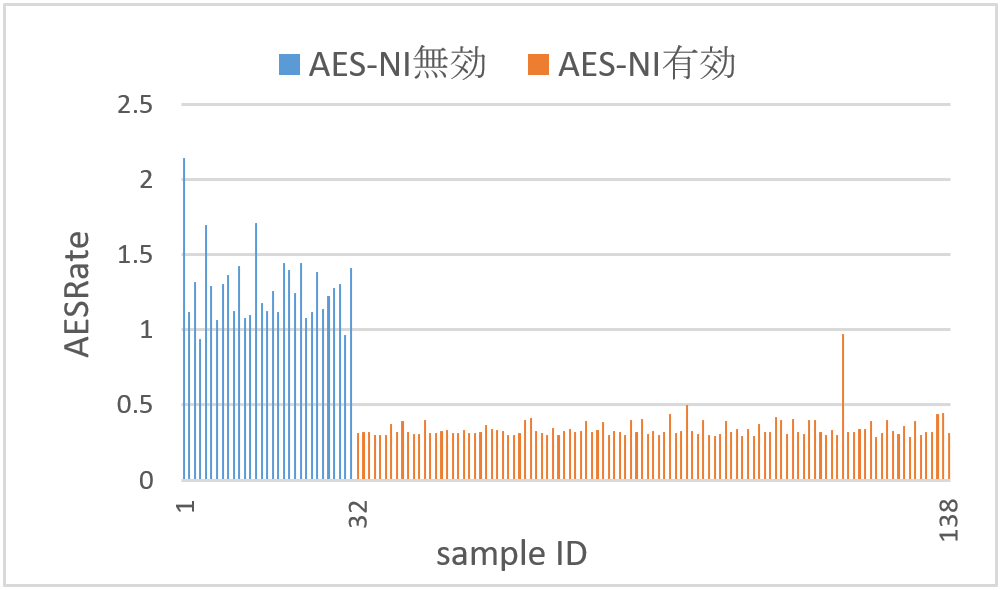
\includegraphics[width=\textwidth,pagebox=cropbox]{fig/aes_rst_chrome.png}
    \subcaption{Chrome}
  \end{minipage}
  \begin{minipage}[b]{0.45\linewidth}
    \centering
    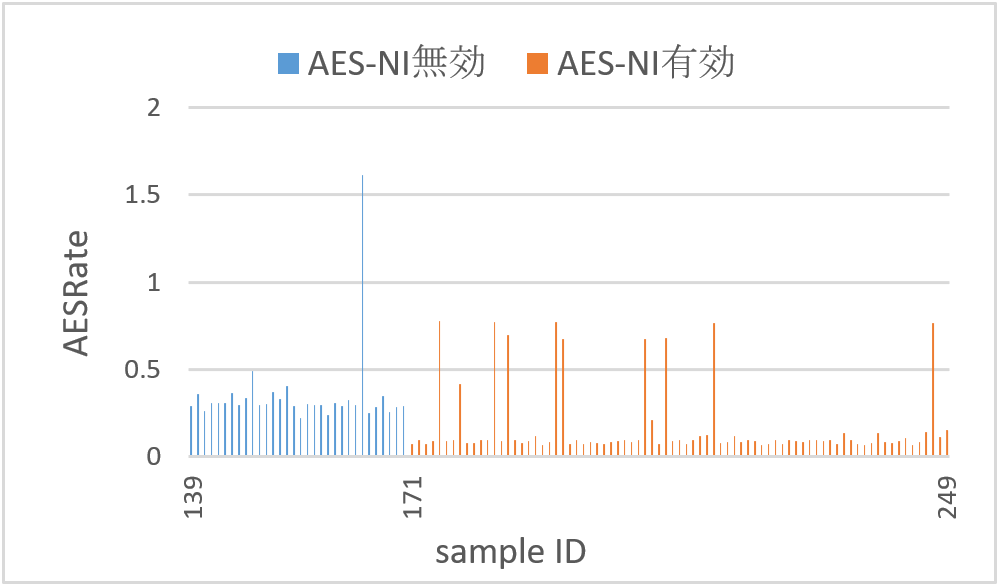
\includegraphics[width=\textwidth,pagebox=cropbox]{fig/aes_rst_firefox.png}
    \subcaption{Firefox}
  \end{minipage}
  \begin{minipage}[b]{0.45\linewidth}
    \centering
    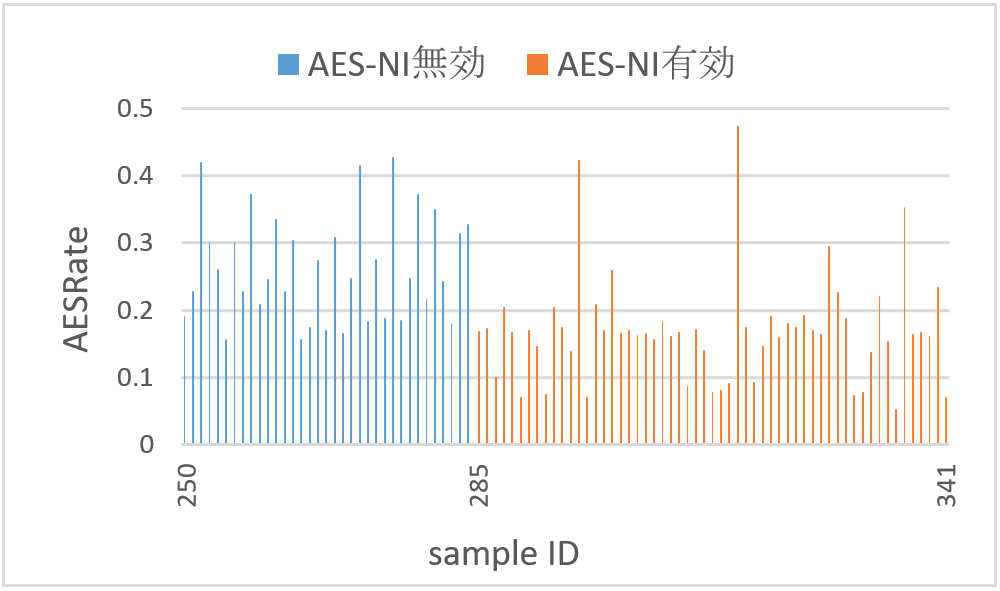
\includegraphics[width=\textwidth,pagebox=cropbox]{fig/aes_rst_ie.png}
    \subcaption{IE}
  \end{minipage}
  \caption{AESRate(採取システム以外)}\label{fig-aes_rst}
\end{figure}

Chromeでは99.28\%,Firefoxでは71.17\%,IEでは77\%の正答率であった.
また,採取時間は平均28.15秒で,最大で243.0秒かかるものもあった.
ブラウザファミリによって正答率に大きな差異があることから,AES-NIが効果的に機能するかは実装によって大きく左右されることが分かる.

採取システムでは処理時間の問題から提案手法よりも少ない時間での計測を行った.
収集結果を図~\ref{fig-aes_rst_sys}に示す.縦軸はAESRateを,横軸はサンプルIDを表す.

\begin{figure}[H]
    \centering
    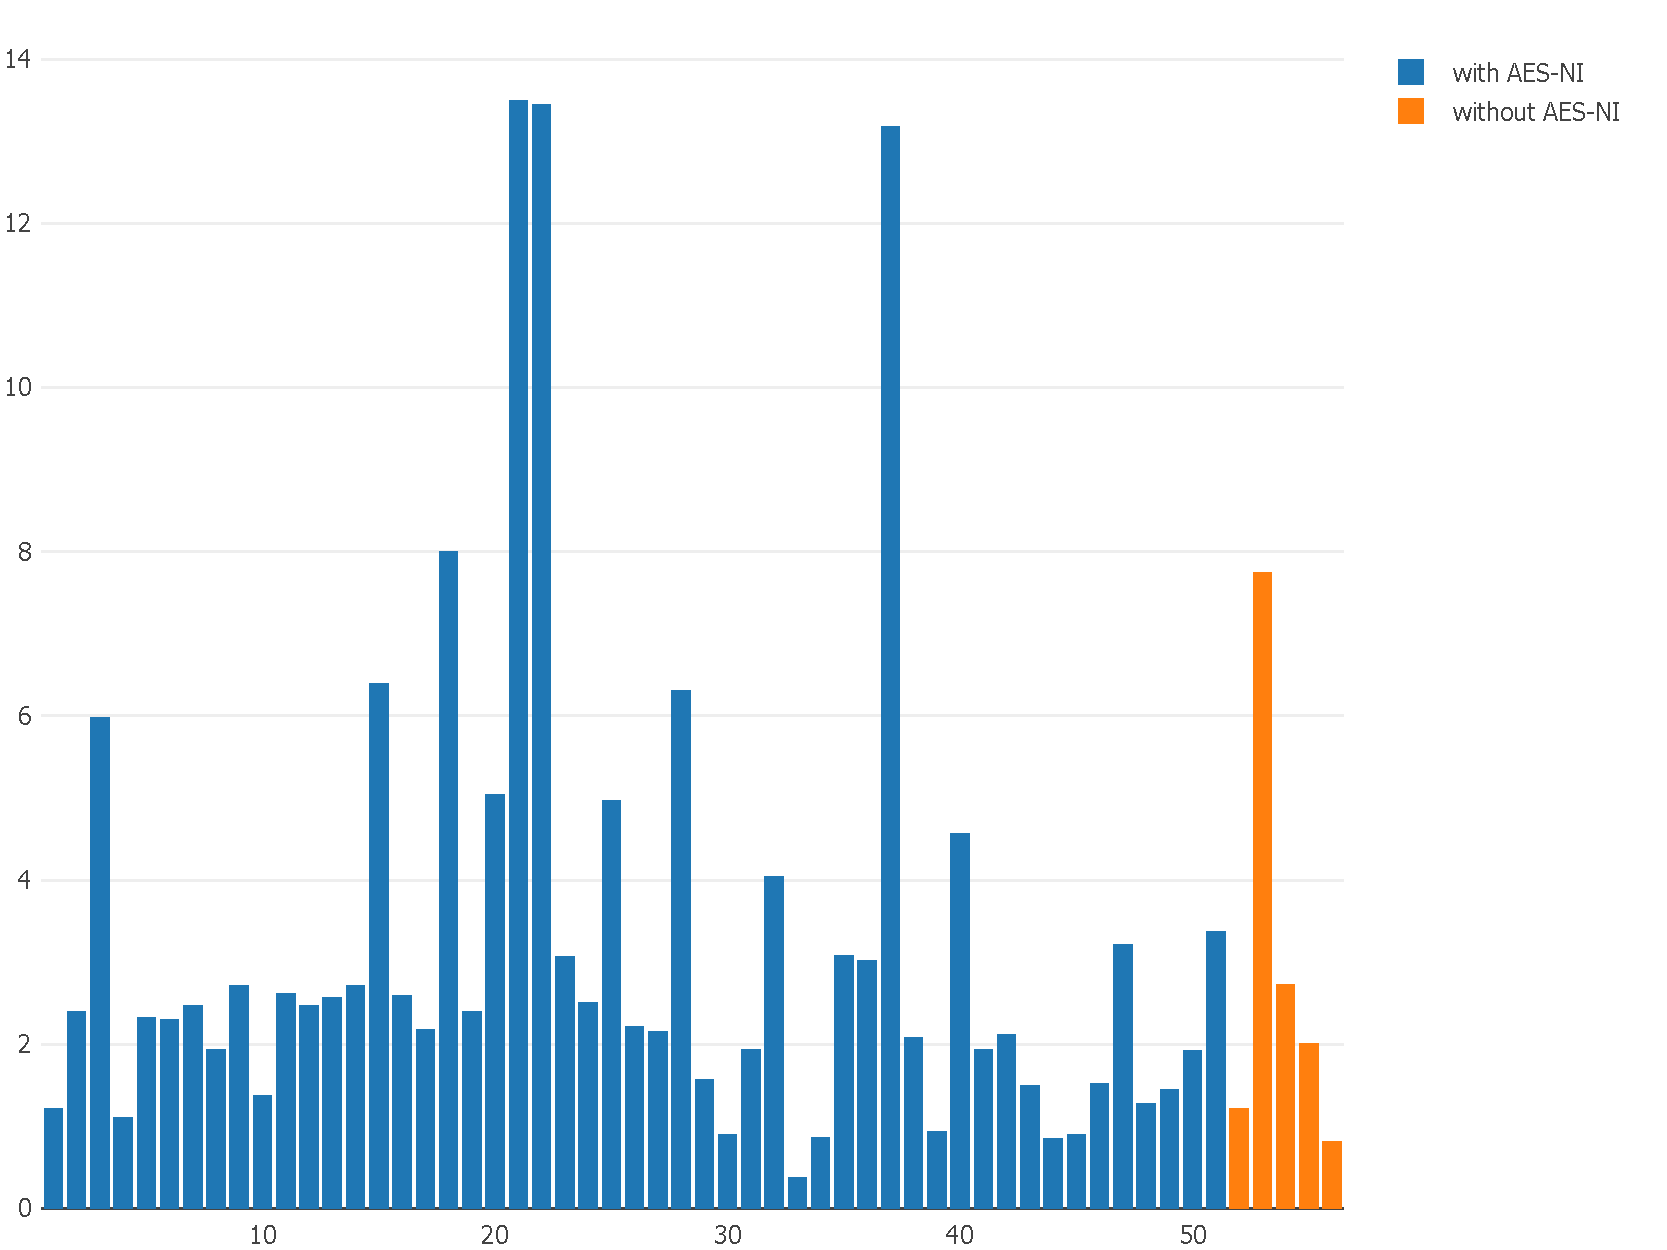
\includegraphics[width=0.6\textwidth,pagebox=cropbox]{fig/aes_rst.pdf}
    \caption{AESRate(採取システム)}
    \label{fig-aes_rst_sys}
\end{figure}

AES-NIへの対応はSMBIOSのType 4におけるVersionから仕様を参照した.
収集したサンプルからは有意差が認められなかった.
これはAES-NIの推定において長い処理時間が必要であることの裏付けとも言える.

\subsection{Turbo Boost}
採取システムを用いないで収集した.
このサンプルは,AES-NIにおける採取システムを用いないで収集したものと同一である.
また,検証法についてもAES-NIと同様である.

結果をブラウザごとに分けて,図~\ref{fig-turbo_rst}に示す.
図の縦軸は$\frac{NavierStokes}{RegExp}$を,横軸はサンプルIDを表しており,Turbo Boostが無効のサンプルと有効なサンプルを色分けして表現している.

\begin{figure}[H]
  \begin{minipage}[b]{0.45\linewidth}
    \centering
    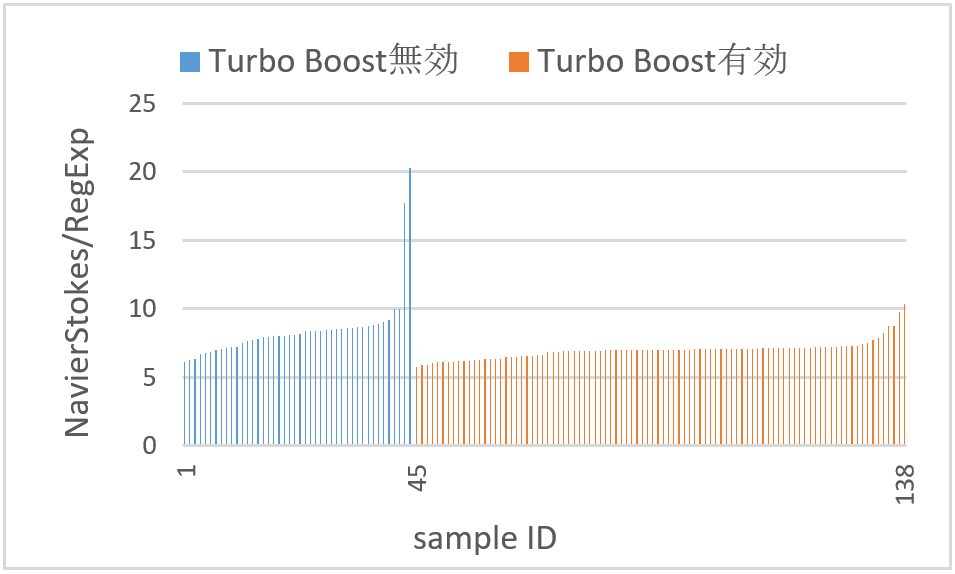
\includegraphics[width=\textwidth,pagebox=cropbox]{fig/turbo_rst_chrome.png}
    \subcaption{Chrome}
  \end{minipage}
  \begin{minipage}[b]{0.45\linewidth}
    \centering
    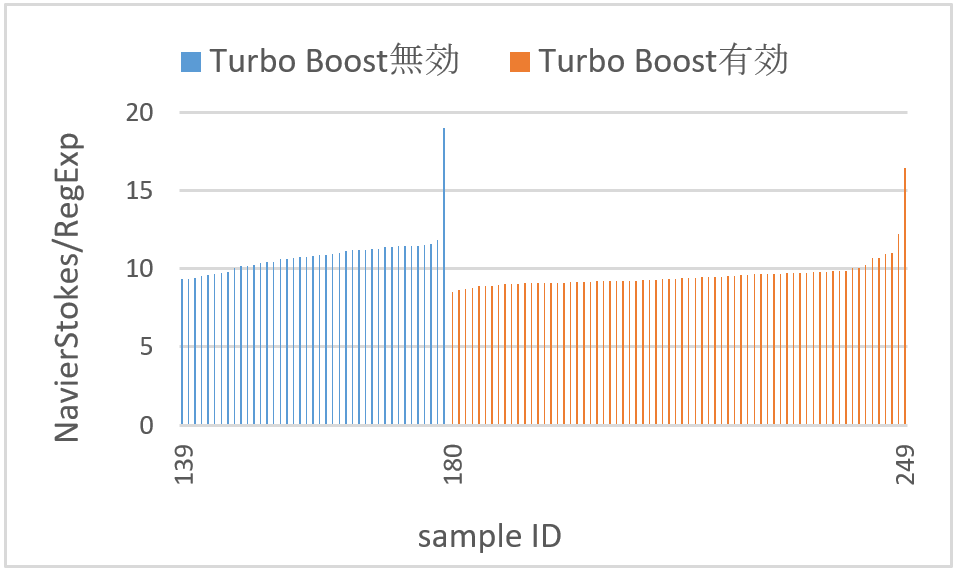
\includegraphics[width=\textwidth,pagebox=cropbox]{fig/turbo_rst_firefox.png}
    \subcaption{Firefox}
  \end{minipage}
  \begin{minipage}[b]{0.45\linewidth}
    \centering
    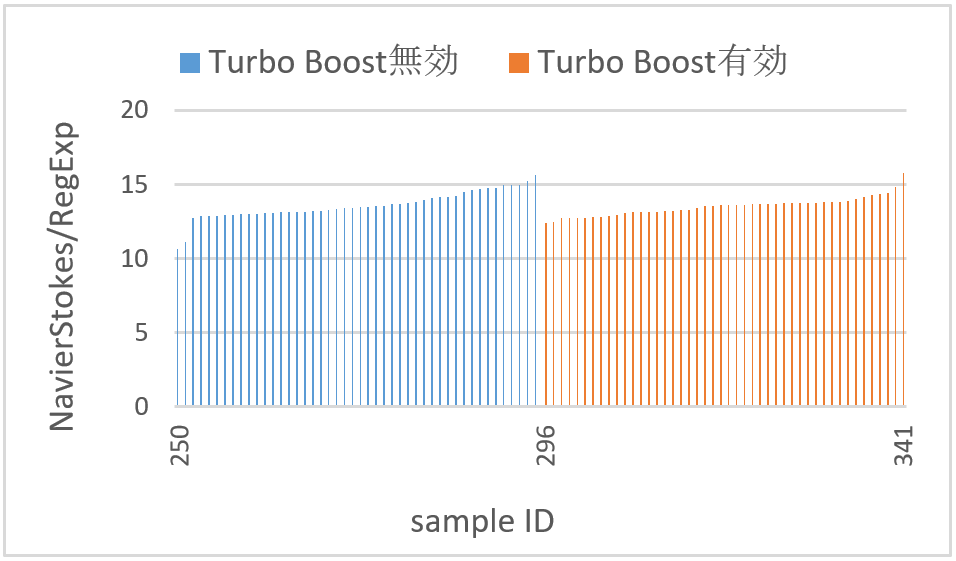
\includegraphics[width=\textwidth,pagebox=cropbox]{fig/turbo_rst_ie.png}
    \subcaption{IE}
  \end{minipage}
  \caption{NavierStokes/RegExp(採取システム以外)}\label{fig-turbo_rst}
\end{figure}

Chromeでは84.78\%,Firefoxでは82.88\%,IEでは55.0\%の正答率であった.
また,採取時間は平均46.91秒で,最大で136.0秒かかるものもあった.
AES-NIと同様に,ブラウザファミリによって正答率に大きな差異があることから,Turbo Boostが効果的に機能するかは実装によって大きく左右されることが分かる.

\subsection{CPUファミリ,マイクロアーキテクチャ,モデルナンバー}
採取システムを用いないで収集した.
合計435のサンプルを収集した.実験協力者はCPUに関する情報とJavaScriptベンチマークの結果を提供する.
提案手法で推定した結果を表~\ref{tb-cpu_family_rst},\ref{tb-cpu_arch_rst}に示す.

\begin{table}[H]
\centering
\caption{CPUファミリの推定結果(採取システム以外)}
\label{tb-cpu_family_rst}
\begin{tabular}{
>{\columncolor[HTML]{C0C0C0}}l llllll}
           & \multicolumn{6}{c}{\cellcolor[HTML]{C0C0C0}真の結果}                                                                                                                                                             \\
予測結果       & \cellcolor[HTML]{C0C0C0}Celeron & \cellcolor[HTML]{C0C0C0}Core 2 Duo & \cellcolor[HTML]{C0C0C0}Core i3 & \cellcolor[HTML]{C0C0C0}Core i5 & \cellcolor[HTML]{C0C0C0}Core i7 & \cellcolor[HTML]{C0C0C0}Pentium \\
Celeron    & \multicolumn{1}{l|}{32}         & \multicolumn{1}{l|}{7}             & \multicolumn{1}{l|}{0}          & \multicolumn{1}{l|}{1}          & \multicolumn{1}{l|}{0}          & 3                               \\ \cline{2-7} 
Core 2 Duo & \multicolumn{1}{l|}{3}          & \multicolumn{1}{l|}{10}            & \multicolumn{1}{l|}{0}          & \multicolumn{1}{l|}{0}          & \multicolumn{1}{l|}{0}          & 3                               \\ \cline{2-7} 
Core i3    & \multicolumn{1}{l|}{0}          & \multicolumn{1}{l|}{0}             & \multicolumn{1}{l|}{23}         & \multicolumn{1}{l|}{8}          & \multicolumn{1}{l|}{0}          & 0                               \\ \cline{2-7} 
Core i5    & \multicolumn{1}{l|}{0}          & \multicolumn{1}{l|}{0}             & \multicolumn{1}{l|}{10}         & \multicolumn{1}{l|}{196}        & \multicolumn{1}{l|}{3}          & 0                               \\ \cline{2-7} 
Core i7    & \multicolumn{1}{l|}{0}          & \multicolumn{1}{l|}{0}             & \multicolumn{1}{l|}{0}          & \multicolumn{1}{l|}{0}          & \multicolumn{1}{l|}{80}         & 0                               \\ \cline{2-7} 
Pentium    & \multicolumn{1}{l|}{4}          & \multicolumn{1}{l|}{2}             & \multicolumn{1}{l|}{0}          & \multicolumn{1}{l|}{0}          & \multicolumn{1}{l|}{0}          & 1                              
\end{tabular}
\end{table}

\begin{table}[H]
\centering
\caption{マイクロアーキテクチャの推定結果(採取システム以外)}
\label{tb-cpu_arch_rst}
\scalebox{0.8}{
\begin{tabular}{
>{\columncolor[HTML]{C0C0C0}}l llllllll}
             & \multicolumn{8}{c}{\cellcolor[HTML]{C0C0C0}真の結果}                                                                                                                                                                                                                                          \\
予測結果         & \cellcolor[HTML]{C0C0C0}Arrandale & \cellcolor[HTML]{C0C0C0}Bay Trail & \cellcolor[HTML]{C0C0C0}Clarkdale & \cellcolor[HTML]{C0C0C0}Conroe & \cellcolor[HTML]{C0C0C0}Haswell & \cellcolor[HTML]{C0C0C0}Ivy Bridge & \cellcolor[HTML]{C0C0C0}Penryn & \cellcolor[HTML]{C0C0C0}Sandy Bridge \\
Arrandale    & \multicolumn{1}{l|}{63}           & \multicolumn{1}{l|}{0}            & \multicolumn{1}{l|}{0}            & \multicolumn{1}{l|}{4}         & \multicolumn{1}{l|}{2}          & \multicolumn{1}{l|}{9}             & \multicolumn{1}{l|}{1}         & 9                                    \\ \cline{2-9} 
Bay Trail    & \multicolumn{1}{l|}{0}            & \multicolumn{1}{l|}{4}            & \multicolumn{1}{l|}{0}            & \multicolumn{1}{l|}{0}         & \multicolumn{1}{l|}{0}          & \multicolumn{1}{l|}{0}             & \multicolumn{1}{l|}{0}         & 1                                    \\ \cline{2-9} 
Clarkdale    & \multicolumn{1}{l|}{0}            & \multicolumn{1}{l|}{0}            & \multicolumn{1}{l|}{3}            & \multicolumn{1}{l|}{0}         & \multicolumn{1}{l|}{0}          & \multicolumn{1}{l|}{0}             & \multicolumn{1}{l|}{0}         & 0                                    \\ \cline{2-9} 
Conroe       & \multicolumn{1}{l|}{4}            & \multicolumn{1}{l|}{0}            & \multicolumn{1}{l|}{0}            & \multicolumn{1}{l|}{4}         & \multicolumn{1}{l|}{0}          & \multicolumn{1}{l|}{0}             & \multicolumn{1}{l|}{0}         & 0                                    \\ \cline{2-9} 
Haswell      & \multicolumn{1}{l|}{0}            & \multicolumn{1}{l|}{1}            & \multicolumn{1}{l|}{0}            & \multicolumn{1}{l|}{0}         & \multicolumn{1}{l|}{28}         & \multicolumn{1}{l|}{5}             & \multicolumn{1}{l|}{0}         & 2                                    \\ \cline{2-9} 
Ivy Bridge   & \multicolumn{1}{l|}{6}            & \multicolumn{1}{l|}{0}            & \multicolumn{1}{l|}{0}            & \multicolumn{1}{l|}{0}         & \multicolumn{1}{l|}{11}         & \multicolumn{1}{l|}{96}            & \multicolumn{1}{l|}{0}         & 7                                    \\ \cline{2-9} 
Penryn       & \multicolumn{1}{l|}{0}            & \multicolumn{1}{l|}{0}            & \multicolumn{1}{l|}{0}            & \multicolumn{1}{l|}{0}         & \multicolumn{1}{l|}{0}          & \multicolumn{1}{l|}{0}             & \multicolumn{1}{l|}{2}         & 0                                    \\ \cline{2-9} 
Sandy Bridge & \multicolumn{1}{l|}{4}            & \multicolumn{1}{l|}{0}            & \multicolumn{1}{l|}{0}            & \multicolumn{1}{l|}{2}         & \multicolumn{1}{l|}{7}          & \multicolumn{1}{l|}{13}            & \multicolumn{1}{l|}{1}         & 83                                   \\ \cline{2-9} 
\end{tabular}
}
\end{table}

推定の正答率は,CPUファミリが88.6\%,マイクロアーキテクチャが75.8\%,モデルナンバーが91.4\%だった.
また,実行時間は平均89.0秒であった.

\subsection{OS}
採取システムで収集した結果を示す.

先行調査\cite{tor_mathtan}において,OSをLinux 64bit,Linux 32bit,Windows,macOSに分類できる演算誤差の数値が報告されている.
収集したサンプルではIEでアクセスしたWindowsの端末においては正しく推定できた.
一方,その他のブラウザでアクセスした端末はWindowsとmacOSの区別が行えない数値を示した.
表~\ref{tb-os_rst}に結果をまとめる.

\begin{table}[H]
    \begin{center}
    \caption{\texttt{Math.tan(-1e300)}の演算誤差(採取システム)}
    \label{tb-os_rst}
        \begin{tabularx}{\linewidth}{X|X}
        OS \& Browser & \texttt{Math.tan(-1e300)} \\ \hline\hline
        Windows \& IE & 4.987183803371 \\ \hline
        Windows or macOS \& Chrome or Firefox or Edge or Safari & 1.4214488238747 \\
        \end{tabularx}
    \end{center}
\end{table}

報告されている演算誤差のみではOSの正確な分類は困難である.通信解析を用いたOS Fingerprintingの方が優れた分類が行えるといえる.

\subsection{CPUのコア数,スレッド数}
採取システムで収集した結果を示す.

先行研究\cite{後藤浩行2013web,桐生直輝2014web}ではIntelのCPUを対象としているので,本論文でもそれに倣ってIntel以外のサンプルを除外した.
収集結果を図~\ref{fig-cpu_rst}に示す.
縦軸は複数のWeb Workerを動作させたときの処理時間を1つのWeb Workerで処理したときの時間で正規化した値を示し,横軸はWeb Workerの数を表している.

\begin{figure}[H]
    \centering
    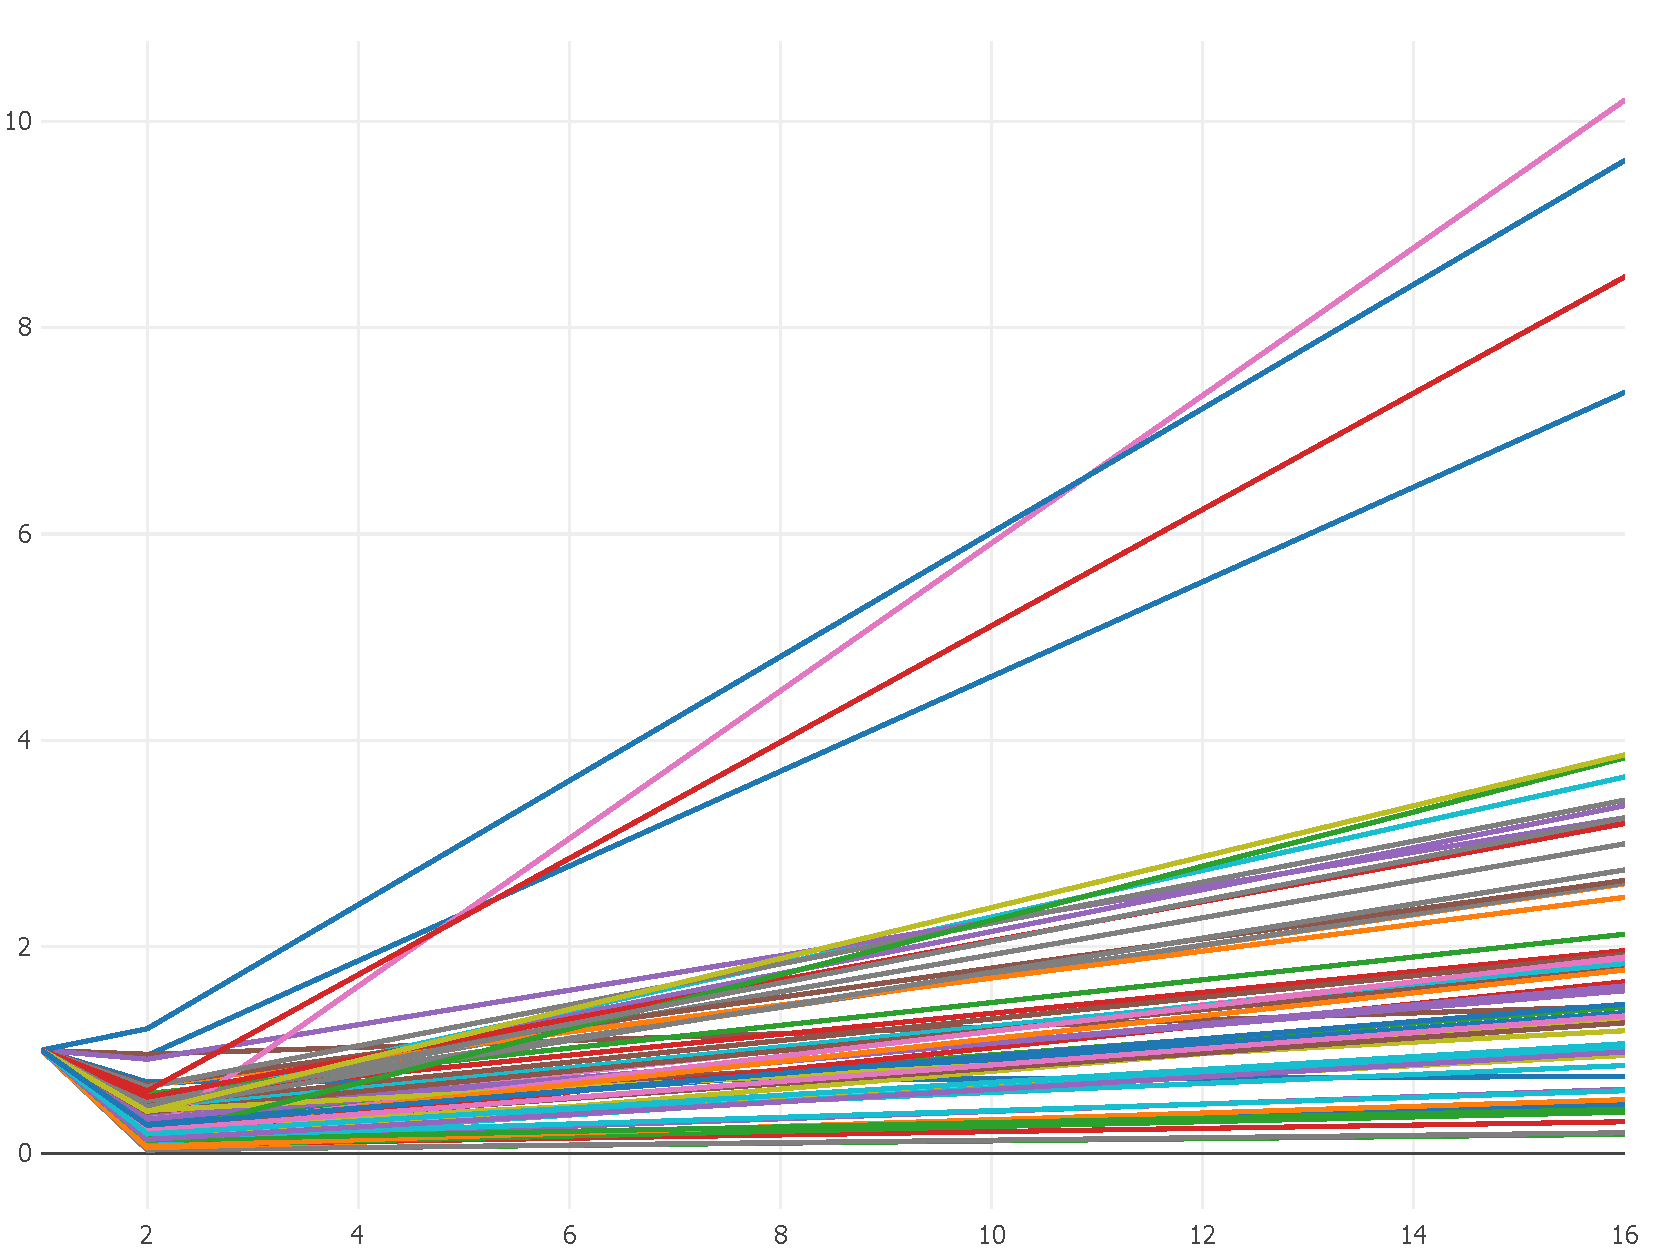
\includegraphics[width=0.6\textwidth,pagebox=cropbox]{fig/cpu_rst.pdf}
    \caption{複数のWeb Workerによる処理速度比(採取システム)}
    \label{fig-cpu_rst}
\end{figure}

4コア8スレッドのような性能の高い端末のデータは顕著な差異が認められる.
一方で,先行研究と同様に,2コア4スレッドや2コア2スレッドの識別は困難であった.


\subsection{バイトオーダー}
採取システムにて収集したサンプルにおいてビッグエンディアン環境はなかった.
ビッグエンディアンは一般的ではなく,これを採用しているアーキテクチャはメインフレームや組み込みマイコンなど一部に限られる.
一方,これらの端末が含まれるサンプルにおいて識別する場合は有用であるといえる.
また,ビッグエンディアン環境については,QEMU\footnote{オープンソースのプロセッサエミュレータ.x86以外のPowerPCやMIPS,SPARCなどのアーキテクチャをエミュレートできる.\url{https://www.qemu.org/}}に代表されるCPUエミュレータを用いることで動作を模倣することができる.これらの環境を使用された場合には正確な判別ができない問題もある.

\subsection{メモリのパフォーマンス}
採取システムにて収集した結果を図~\ref{fig-memory_rst}に示す.
縦軸は\texttt{Typed Array}へのアクセス時間を基準とするアクセス速度で正規化した値を示し,横軸はアクセスした\texttt{Typed Array}のサイズを示している.

\begin{figure}[H]
    \centering
    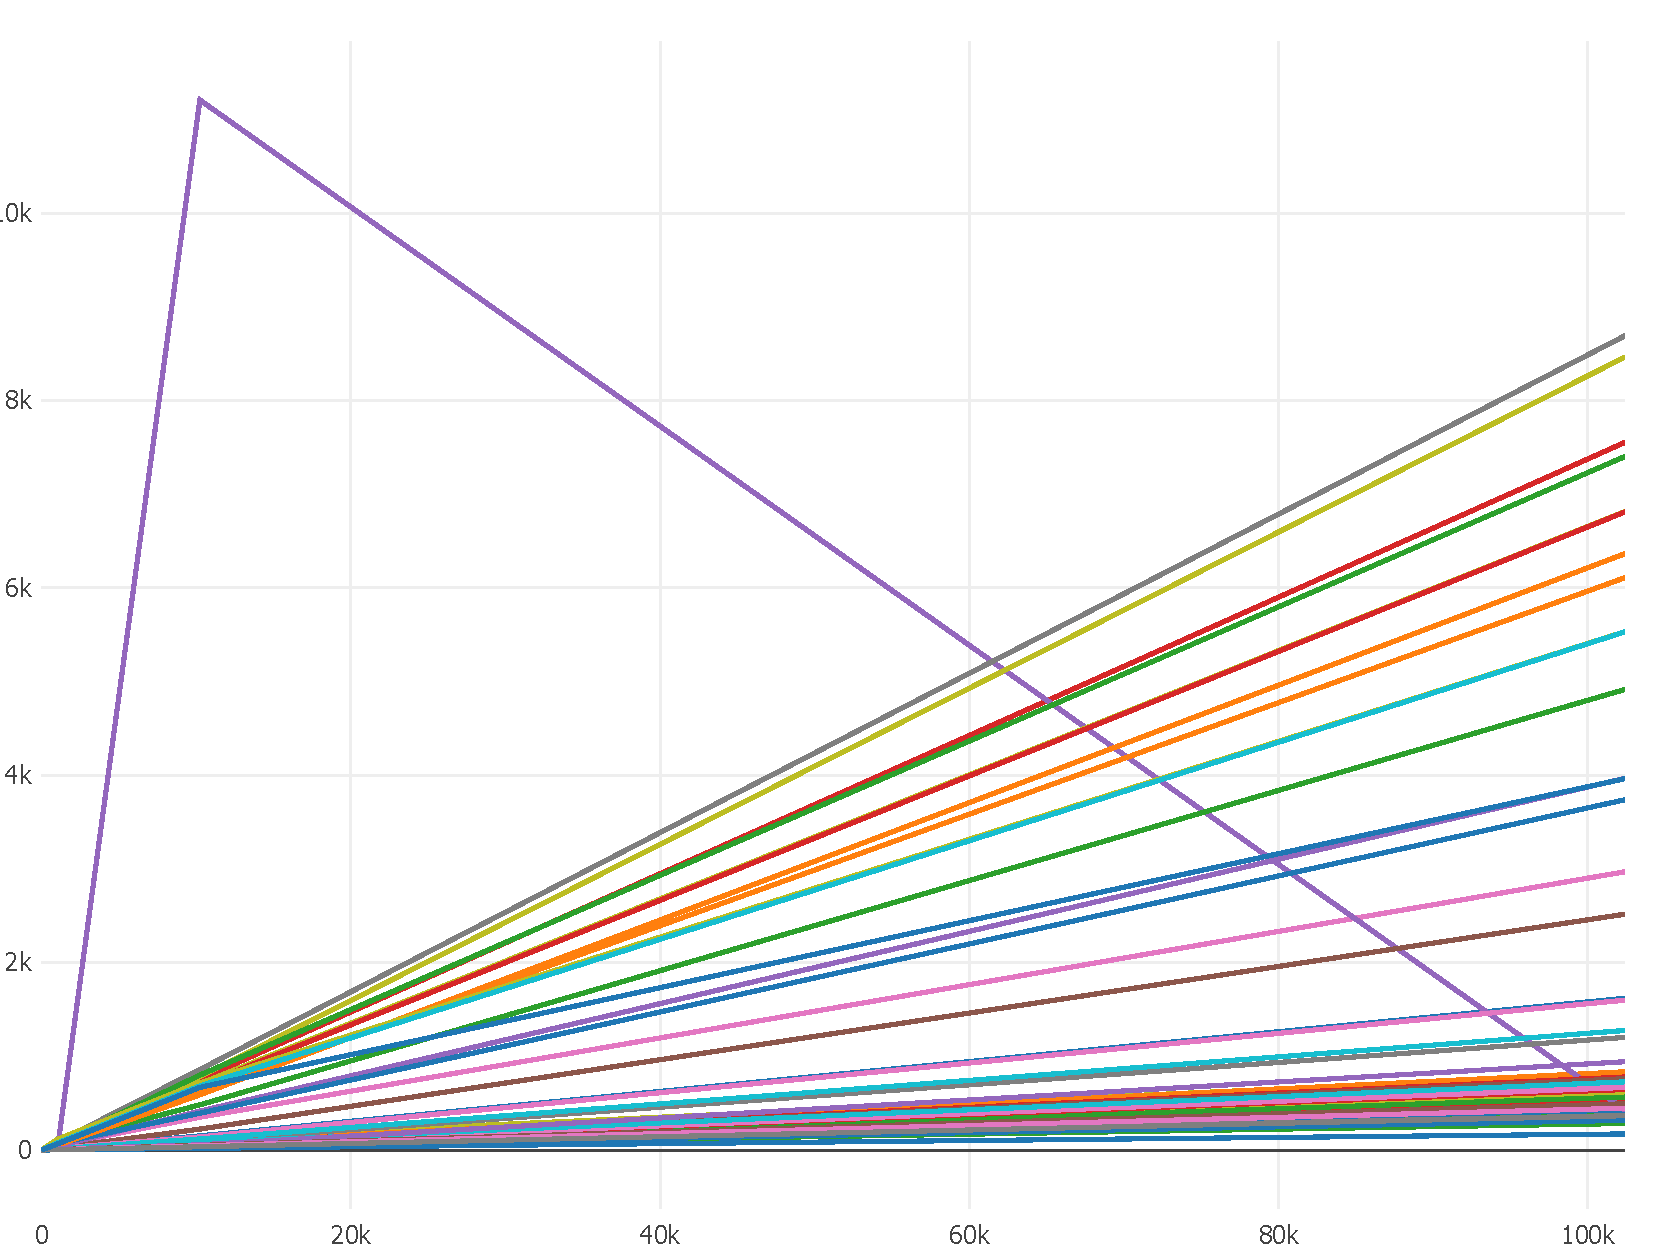
\includegraphics[width=0.6\textwidth,pagebox=cropbox]{fig/memory_rst.pdf}
    \caption{\texttt{Typed Array}へのサイズごとのアクセス速度(採取システム)}
    \label{fig-memory_rst}
\end{figure}

ここで,メモリ操作はブラウザによって実装方法が異なることから,ブラウザによる差異を緩和する必要があることがわかった.
ブラウザごとのアクセスに要した平均時間を説明変数に加え,SMBIOSのType 17から採取したメモリのクロック周波数を回帰分析した.
その結果,決定係数が0.12となった.
この収集結果からは,メモリのパフォーマンスの推定が困難であったが,端末ごとに異なる値を示すことから\fp~への適用は考えられる.

\subsection{GPU}
採取システムにて収集した結果を示す.

先行研究\cite{mowery2012pixel}で示された手法を用いて,採取したものからPCI接続可能なGPUを表しているものを表~\ref{tb-gpu_rst}にまとめた.

\begin{table}[h]
    \begin{center}
    \caption{WebGL APIにて採取したGPU一覧(採取システム)}
    \label{tb-gpu_rst}
        \begin{tabularx}{\linewidth}{|X|} \hline
            ANGLE (NVIDIA GeForce GTX 750 Ti Direct3D11 vs\_5\_0 ps\_5\_0) \\ \hline
            ANGLE (NVIDIA GeForce GT 520 Direct3D11 vs\_5\_0 ps\_5\_0) \\ \hline
            ANGLE (NVIDIA GeForce GTX 960 Direct3D11 vs\_5\_0 ps\_5\_0) \\ \hline
            ANGLE (NVIDIA GeForce GTX 550 Ti Direct3D11 vs\_5\_0 ps\_5\_0) \\ \hline
            ANGLE (AMD Radeon HD 5670 Direct3D11 vs\_5\_0 ps\_5\_0) \\ \hline
        \end{tabularx}
    \end{center}
\end{table}

表~\ref{tb-gpu_rst}に示した端末のSMBIOSのType 9を確認したところ,1つを除いて他のすべてのサンプルはPCIe x16がIn Useであった.例外的に1つのサンプルはType 9の情報が存在せず,PCI接続スロットがないのにもかかわらずPCI接続が必要なGPUを使用しているようであった.

\subsection{GPUパフォーマンス}
採取システムにて収集した結果を示す.

結果を図~\ref{fig-gpgpu_rst}に示す.
横軸はサンプルのIDを表し,縦軸はGPGPUによる演算時間をCPUによる演算時間で正規化したものである.

\begin{figure}[H]
    \centering
    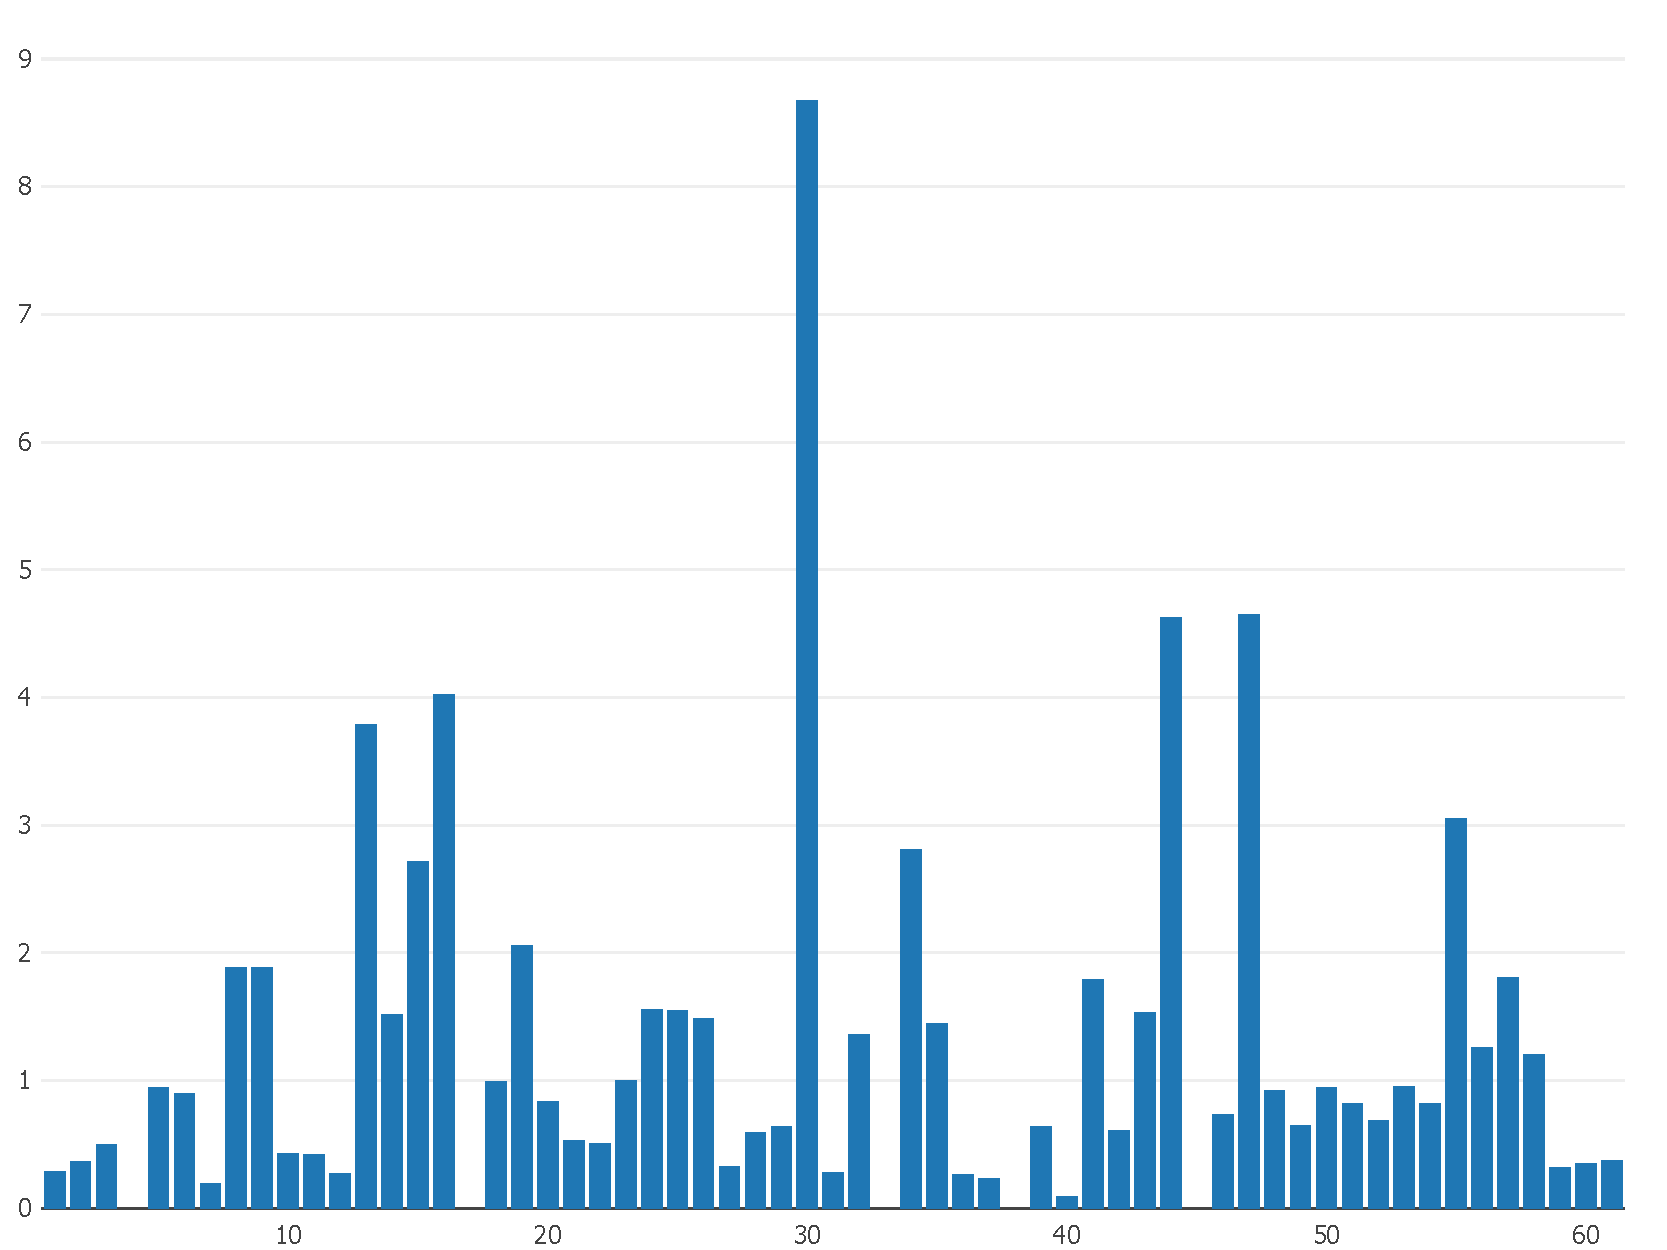
\includegraphics[width=0.6\textwidth,pagebox=cropbox]{fig/gpgpu_rst.pdf}
    \caption{GPGPUによる演算速度の比率(採取システム)}
    \label{fig-gpgpu_rst}
\end{figure}

端末ごとにバラツキが出ることはわかるが,PCI接続されたGPUとの相関は見られなかった.
高い比率を示したサンプル(つまり,GPGPUパフォーマンスが高い)の中には,GPUで処理が行えない端末向けにCPUのみでレンダリング速度を向上させるSwiftShader\footnote{Googleが開発している,CPUのみで描画処理を高速に動作させるライブラリ.Chromeでは利用可能なGPUがない場合には自動でこの機能が有効となる.\url{https://github.com/google/swiftshader}}を実装しているブラウザでアクセスしている端末もあった.
また,CPUにオンチップで搭載されているGPUについても性能が向上している.
ただし,レンダリング性能との関係性は依然あるので,\fp~における活用は考えられる.
